\chapter{Subjective validation of synthesis method}\label{chapter:test}\todo{From paper. Rewrite}

\section{Introduction}
In chapter \ref{chapter:tool} an overview was given of the auralisation tool. A
propagation model for aircraft sound was developed but still missing is an
emission model. An algorithm was presented for extracting select features from
recordings and these features could potentially be used for the development of
an (semi-)empirical emission model.

This chapter describes a listening test that was conducted. The purpose of the
test was to determine whether the auralisation tool produces auralisations that
sound similar to recordings. Because the available data sets permits simulating
and comparing different aircraft types, the purpose was also to test whether
participants can distinguish between aircraft types.

\section{Method}

The goal of the listening test was to determine whether the auralisations sound
similar to the recordings they were based on. Participants were presented with
pairs of stimuli and asked to rate how similar they sounded.

% \todo{explain why this method is chosen? Explain other available methods?}
% One can think of multiple methods to
% determine the similarity. The MUSHRA (MUltiple Stimuli with Hidden Reference and
% Anchor) test is methodology used for evaluating audio quality \cite{}, and has also been used for determining the plausibility of synthesised vehicle pass-by sounds when compared to recordings \cite{Southern2016}.

Eight different stimuli were considered and they were 12 seconds long.
Because the sounds vary considerably over time, they were each split into parts
of 4 seconds, corresponding to the approach, fly-over and distancing. For each
part all combinations were considered. Each part therefore consisted of 28 pairs
of stimuli of four seconds.

Of the eight stimuli four were recordings, and four were auralisations with each
of them based on one of the recordings. Two aircraft types were considered, an
A320 and a RJ1H, and two events per aircraft type.
% The recordings were made close to the airport. \todo{this sentence can be dropped if we have a Measurements section}
% with the aircraft passing by at approximately 90 meters.
Headphones were used and HRTF's were not included.

Because similarity is relative, an anchor is typically used. In this test the
participants were for each part first given the set of stimuli, in order to
become familiar with the type of sounds and the spread in the sounds of that
part, and then continued with rating the pairs. The rating was done on an eleven
point Likert scale. The left side of the scale said ``not so much'' and the right
side ``very much''. The scale was not numbered.


\section{Results}
The results of the participants were scaled linearly from 0 to 1 with 0
correspond to ``not so much'' and 1 corresponding to ``very much''. Since not
all participants used the full scale, they were rescaled per participant to use
the full scale. There were 17 participants, all graduate students, and of which
the majority studied acoustics. The results that are shown are obtained after
joining the data of all participants and all three test parts.

Figure \ref{fig:ratings_recordings} shows the similarity ratings grouped per
aircraft combination, considering only recordings. Figure
\ref{fig:ratings_simulations} shows the similarity ratings grouped per
aircraft combination, but now for the auralisations.
Figures \ref{fig:ratings_A320} and \ref{fig:ratings_RJ1H} show
for respectively the A320 and the RJ1H the similarity ratings grouped per pairs
of stimuli type, that is, recordings and/or simulations.
The listening test and results can be found at respectively \cite{Rietdijk2017a} and \cite{Rietdijk2017b}.

% \begin{figure}[H]
%   \centering
%   \includegraphics[]{figure_ratings}
%   \caption{Similarity ratings for different groups.}
%   \label{fig:ratings
% \end{figure}

\todo{group figures in grid}

\begin{figure}[H]
  \centering
  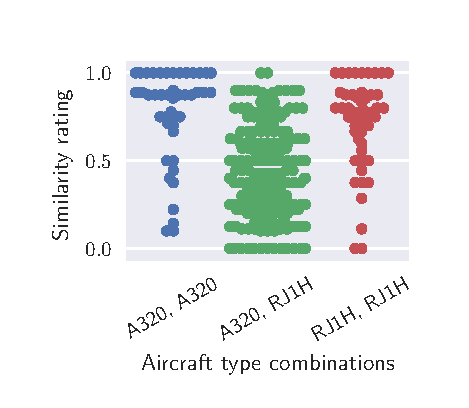
\includegraphics[]{../figures/manual/auralisation-paper/figure1_ratings_recordings}
  \caption{Similarity ratings for the recordings grouped by aircraft type.}
  \label{fig:ratings_recordings}
\end{figure}

\begin{figure}[H]
  \centering
  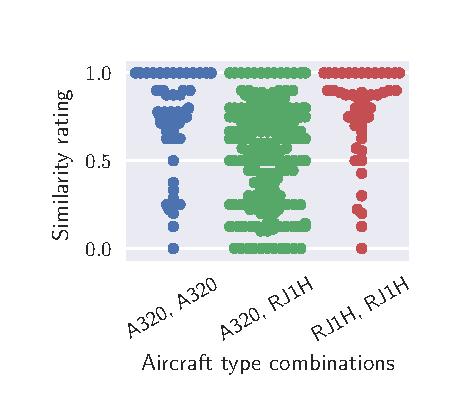
\includegraphics[]{../figures/manual/auralisation-paper/figure2_ratings_simulations}
  \caption{Similarity ratings for the auralisations grouped by aircraft type.}
  \label{fig:ratings_simulations}
\end{figure}

\begin{figure}[H]
  \centering
  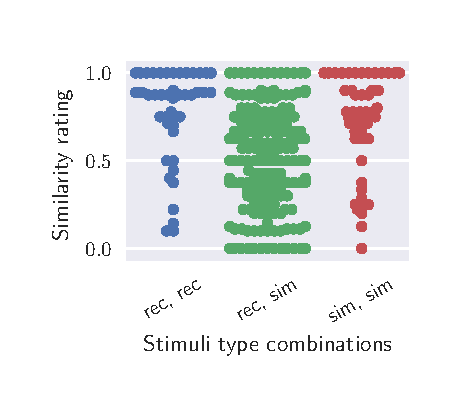
\includegraphics[]{../figures/manual/auralisation-paper/figure3_ratings_A320}
  \caption{Similarity ratings for the A320 grouped by stimuli type combinations.}
  \label{fig:ratings_A320}
\end{figure}

\begin{figure}[H]
  \centering
  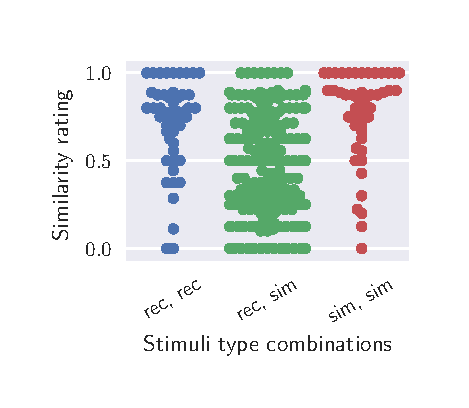
\includegraphics[]{../figures/manual/auralisation-paper/figure4_ratings_RJ1H}
  \caption{Similarity ratings for the RJ1H grouped by stimuli type combinations.}
  \label{fig:ratings_RJ1H}
\end{figure}

The ratings were obtained for three different parts of the stimuli, ``start'',
``center'' and ``end'', and that allows us to also group the ratings by each of
these parts. Figures \ref{fig:ratings_part_A320} and \ref{fig:ratings_part_RJ1H}
show the similarity ratings for respectively the A320 and RJ1H grouped per
stimuli type combination and per stimuli part. A Tukey boxplot is used to
improve the clarity of the figure.

\begin{figure}[H]
  \centering
  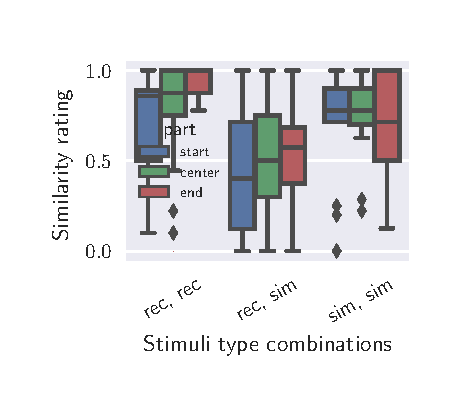
\includegraphics[]{../figures/manual/auralisation-paper/figure5_ratings_part_A320}
  \caption{Similarity ratings for the A320 grouped by stimuli type combinations and stimuli part.}
  \label{fig:ratings_part_A320}
\end{figure}

\begin{figure}[H]
  \centering
  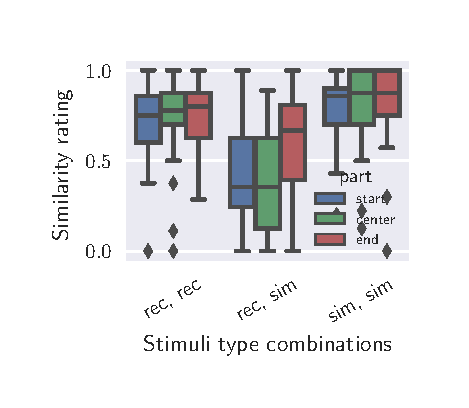
\includegraphics[]{../figures/manual/auralisation-paper/figure6_ratings_part_RJ1H}
  \caption{Similarity ratings for the RJ1H grouped by stimuli type combinations and stimuli part.}
  \label{fig:ratings_part_RJ1H}
\end{figure}

Participants mentioned they noted larger differences at especially the beginning
of the events (``start`` parts) and also at the end of the events (``end`` parts). A
common answer to the question how many aircraft they heard was ``two or three``.
Occasionally, the answer would start at ``two`` but go to ``two or more`` after they
were told they were listening to not only recordings but also simulations. Some
participants were surprised when told that simulations were included,
others said they had thought so, and a few of the participants were already
aware the test was possibly going to contain simulations.

\section{Discussion}
As can be seen in Figure \ref{fig:ratings_recordings}, the A320's are judged to be very
similar to each other, and the RJ1H's as quite similar to each other. The A320's
are not rated as very similar to the RJ1H's and therefore we conclude that the
participants can discriminate between the two aircraft types.

In the case of the auralisations, Figure \ref{fig:ratings_simulations}, the
participants can also discriminate between the aircraft types, but now the
RJ1H's are judged to be relatively more similar than the A320's. Compared to the recordings
the difference between the A320's and the RJ1H's is slightly smaller.

% One might argue from these findings that the whole set of auralisations is more similar than the set of recordings.

Figures \ref{fig:ratings_A320} and \ref{fig:ratings_RJ1H} show
as additional information how similar the auralisations are to the recordings.
The groups ``(rec, sim)'' contain pairs consisting of a recording and an
auralisation. The similarity ratings for these two groups are similar to the
``(A320, RJ1H)'' groups in Figures \ref{fig:ratings_recordings} and
\ref{fig:ratings_simulations}. Therefore, it would appear that listeners can
discriminate between aircraft types, but that the auralisations are considered
to be of different aircraft types than the recordings they're based on.

Figures \ref{fig:ratings_part_A320} and \ref{fig:ratings_part_RJ1H} show the
same data but now further grouped by stimuli part. Judging from Figure
\ref{fig:ratings_part_A320} there appears to be a relative large dissimilarity
between the ``start'' parts of the A320 recordings and also between the ``end''
parts of the A320 auralisations. The groups ``(rec, rec)'' and ``(sim, sim)''
consist however of only 17 data points each whereas the ``(rec, sim)'' group
has 68 data points.

The participants mentioned relatively larger differences in the stimuli that
correspond to the approach of the aircraft (``start`` stimuli). During the
approach the tonal components are clearly audible compared to other parts of the
events due to the directivity. The feature-extraction algorithm was known to
underestimate the power and bandwidth of the blade passing frequency and its
harmonics because the algorithm was tuned for the Buzz-Saw tones. Therefore, a
likely explanation is that this underestimation of power and bandwidth is
causing audible differences between recordings and auralisations.
